\documentclass[aspectratio=169,11pt]{beamer}

\usepackage[T1]{fontenc}
\usepackage[utf8]{inputenc}
\usepackage{graphicx}
\usepackage{booktabs}
\usepackage{array}
\usepackage{tabularx}
\usepackage{tikz}
\usepackage{xcolor}
\usepackage{amsmath}

\setbeamertemplate{navigation symbols}{}
\setbeamertemplate{blocks}[rounded][shadow=true]

\definecolor{oublack}{HTML}{121212}
\definecolor{ougold}{HTML}{B59A57}
\definecolor{ougoldlight}{HTML}{E3D4A5}
\definecolor{oustone}{HTML}{F5F1E8}
\definecolor{ougray}{HTML}{5C5A56}
\definecolor{ouline}{HTML}{D8CCAB}
\definecolor{tsnavy}{HTML}{0E172A}
\definecolor{tsblue}{HTML}{1F4E79}
\definecolor{tsteal}{HTML}{0F766E}
\definecolor{tssoft}{HTML}{F7F9FC}
\definecolor{tsmuted}{HTML}{52606D}
\definecolor{tswarn}{HTML}{A56A00}

\setbeamercolor{structure}{fg=ougold}
\setbeamercolor{title}{fg=oublack}
\setbeamercolor{subtitle}{fg=ougray}
\setbeamercolor{author}{fg=ougray}
\setbeamercolor{date}{fg=ougray}
\setbeamercolor{normal text}{fg=oublack,bg=white}
\setbeamercolor{block title}{fg=white,bg=oublack}
\setbeamercolor{block body}{fg=oublack,bg=tssoft}
\setbeamercolor{frametitle}{fg=white,bg=oublack}
\setbeamercolor{footline}{fg=white,bg=oublack}

\newcommand{\oaklandwordmarkpath}{../../frontend/public/ou-oakland-logo.png}
\newcommand{\oaklandlogopath}{images/oakland_university_logo-freelogovectors.net_.png}
\newcommand{\oaklandbrandbadge}{%
  \tikz[baseline=(box.base)]{
    \node[rounded corners=4pt, fill=oustone, inner xsep=3pt, inner ysep=2pt] (box) {%
      \IfFileExists{\oaklandlogopath}{\includegraphics[height=0.40cm]{\oaklandlogopath}}{\scriptsize\bfseries OU}%
    };
  }%
}

\setbeamertemplate{background canvas}{%
  \begin{tikzpicture}[remember picture,overlay]
    \fill[white] (current page.south west) rectangle (current page.north east);
    \fill[oustone] (current page.south west) rectangle ([yshift=0.38cm]current page.south east);
    \fill[ougold,opacity=0.08] ([xshift=1.0cm,yshift=6.7cm]current page.south west) circle (2.0cm);
    \fill[tsblue,opacity=0.06] ([xshift=12.2cm,yshift=6.8cm]current page.south west) circle (2.3cm);
    \fill[tsteal,opacity=0.05] ([xshift=11.4cm,yshift=1.1cm]current page.south west) circle (1.5cm);
    \draw[ouline,line width=0.35pt] ([yshift=0.38cm]current page.south west) -- ([yshift=0.38cm]current page.south east);
    \draw[ouline!55, line width=0.2pt, opacity=0.35] ([xshift=0.65cm,yshift=0.9cm]current page.south west) grid[xstep=1.05cm,ystep=0.78cm] ([xshift=-0.65cm,yshift=-0.95cm]current page.north east);
  \end{tikzpicture}
}

\setbeamertemplate{frametitle}{%
  \nointerlineskip
  \begin{beamercolorbox}[wd=\paperwidth,ht=1.05cm,dp=0.22cm,leftskip=0.55cm,rightskip=0.3cm]{frametitle}
    
\begin{tikzpicture}[remember picture,overlay]
      \fill[oublack] (0,0) rectangle (\paperwidth,1.28);
      \fill[ougold] (0,0) rectangle (\paperwidth,0.09);
      \fill[ougoldlight,opacity=0.55] (0.55,0.32) rectangle (4.85,0.36);
    \end{tikzpicture}
    \vspace*{0.1cm}\insertframetitle
  \end{beamercolorbox}
}

\setbeamertemplate{footline}{%
  \leavevmode%
  \hbox{%
    \begin{beamercolorbox}[wd=\paperwidth,ht=0.54cm,dp=0.15cm,leftskip=0.38cm,rightskip=0.3cm]{footline}
      \begin{minipage}[c][0.54cm][c]{0.70\paperwidth}
        \centering\raisebox{0.265cm}{\scriptsize\bfseries Oakland University\hspace{0.55em}{\scriptsize School of Engineering and Computer Science}}
      \end{minipage}%
      \begin{minipage}[c][0.54cm][c]{0.14\paperwidth}
        \centering\raisebox{0.265cm}{\scriptsize\insertframenumber/\inserttotalframenumber}
      \end{minipage}%
      \begin{minipage}[c][0.54cm][c]{0.12\paperwidth}
        \centering\raisebox{0.28cm}{\oaklandbrandbadge}
      \end{minipage}%
    \end{beamercolorbox}%
  }%
}

\newcommand{\slidelead}[1]{%
  {\color{tsmuted}\footnotesize #1\par}
  \vspace{0.35em}
}

\newcommand{\metricpill}[2]{%
  \tikz[baseline=-0.65ex]\node[rounded corners=8pt, fill=#1, text=white, inner xsep=8pt, inner ysep=4pt, font=\scriptsize\bfseries]{#2};%
}

\newcommand{\statcard}[2]{%
  \begin{beamercolorbox}[wd=\linewidth,rounded=true,shadow=true,sep=0.18cm]{block body}
    {\scriptsize\textcolor{tsmuted}{#1}}\par
    \vspace{0.22em}
    {\large\bfseries #2}
  \end{beamercolorbox}
}

\title{TrustStack}
\subtitle{A Local-First, Evidence-Grounded Evaluation Standard for Trustworthy AI}
\author{Cordell Stonecipher}
\institute{Oakland University}
\date{CSI-4130/5130 Artificial Intelligence}

\begin{document}

\begin{frame}[plain]
  
\begin{tikzpicture}[remember picture,overlay]
    \fill[oustone] (current page.south west) rectangle (current page.north east);
    \fill[ougold] (current page.north west) rectangle ([xshift=3.0cm,yshift=-0.14cm]current page.north west);
    \fill[ougold,opacity=0.12] ([xshift=11.0cm,yshift=5.8cm]current page.south west) circle (2.4cm);
    \fill[tsteal,opacity=0.10] ([xshift=1.0cm,yshift=1.0cm]current page.south west) circle (1.8cm);
    \draw[ouline,line width=0.7pt] ([xshift=0.62cm,yshift=0.78cm]current page.south west) rectangle ([xshift=-0.62cm,yshift=-0.78cm]current page.north east);
  \end{tikzpicture}
  \vspace*{0.8cm}
  {\color{oublack}\fontsize{24}{28}\selectfont\bfseries \inserttitle\par}
  \vspace{0.4em}
  {\color{ougray}\large \insertsubtitle\par}
  \vspace{0.8em}
  {\color{oublack}\normalsize \insertauthor\par}
  {\color{ougray}\small School of Engineering and Computer Science\par}
  {\color{ougray}\small \insertdate\par}
  \vfill
  \vspace*{1.5cm}
  \begin{center}
    \IfFileExists{\oaklandwordmarkpath}{\includegraphics[width=0.2\linewidth]{\oaklandwordmarkpath}}{\Large Oakland University}
  \end{center}
\end{frame}

\begin{frame}[shrink=8]{1. Introduction and Problem Setting}
  \vspace*{-0.28cm}
  \begin{columns}[T,totalwidth=\textwidth]
    \column{0.58\textwidth}
    \slidelead{TrustStack starts from a simple problem: a fluent answer is not enough when a user must decide whether an AI output is safe, supported, and auditable before using it.}
    \begin{block}{Research question}
      How can a user judge whether an AI answer is trustworthy when conventional chat interfaces expose fluency but hide evidence quality, contradiction risk, and review conditions?
    \end{block}
    \begin{block}{Project thesis}
      TrustStack reframes trust as an evidence-grounded evaluation task. It turns trust into a structured review artifact built from evidence, scoring, risk signals, and explanation.
    \end{block}
    \column{0.38\textwidth}
    \statcard{Core task}{Grounded trust review}
    \vspace{0.45em}
    \statcard{Primary risk}{Unsupported confidence}
    \vspace{0.45em}
    \statcard{Decision basis}{Evidence + diagnostics}
  \end{columns}
\end{frame}

\begin{frame}{2. Related Work and Contribution}
  \slidelead{Most AI systems focus on generating answers. TrustStack focuses on checking whether those answers deserve trust.}
  \begin{columns}[T,totalwidth=\textwidth]
    \column{0.32\textwidth}
    \begin{block}{RAG systems}
      Pull evidence before answering.
    \end{block}
    \column{0.32\textwidth}
    \begin{block}{Reliability research}
      Good sounding text can still be wrong.
    \end{block}
    \column{0.32\textwidth}
    \begin{block}{Evaluation frameworks}
      Teams need repeatable scoring and reports.
    \end{block}
  \end{columns}
  \vspace{0.6em}
  \begin{block}{TrustStack contribution}
      One local-first workflow that checks evidence, scores trust, and produces report-ready outputs.
  \end{block}
\end{frame}

\begin{frame}{3. Data}
  \slidelead{TrustStack evaluates AI with both real user evidence and benchmark data.}
  \begin{columns}[T,totalwidth=\textwidth]
    \column{0.48\textwidth}
    \begin{block}{Live evidence path}
      \small
      \begin{itemize}
        \item PDF, DOCX, TXT, and Markdown uploads
        \item Split into chunks and stored in MongoDB
        \item Used for grounded question answering
      \end{itemize}
    \end{block}
    \column{0.48\textwidth}
    \begin{block}{Benchmark path}
      \small
      \begin{itemize}
        \item Seven synthetic stress tests
        \item Public slices from SciFact and HotpotQA
        \item Same scoring logic across all cases
      \end{itemize}
    \end{block}
  \end{columns}
  \vspace{0.6em}
  \begin{center}
    \metricpill{tsteal}{User uploads}\hspace{0.5em}
    \metricpill{tsblue}{Synthetic stress tests}\hspace{0.5em}
    \metricpill{tswarn}{External benchmarks}
  \end{center}
\end{frame}

\begin{frame}{4. Methods and System Architecture}
  \slidelead{The system follows a simple five-step pipeline so users can see where trust is gained or lost.}
  \begin{block}{Pipeline}
    \centering
    \metricpill{tsblue}{1. Ingest}\hspace{0.4em}
    \metricpill{tsteal}{2. Retrieve}\hspace{0.4em}
    \metricpill{ougold}{3. Generate}\hspace{0.4em}
    \metricpill{tsblue}{4. Evaluate}\hspace{0.4em}
    \metricpill{tsteal}{5. Review / Export}
  \end{block}
  \vspace{0.6em}
  \begin{columns}[T,totalwidth=\textwidth]
    \column{0.48\textwidth}
    \begin{block}{Implementation}
      \small
      \begin{itemize}
        \item MongoDB stores documents, chunks, and run history
        \item Retrieval uses vector search or lexical fallback
        \item Answers remain grounded with deterministic fallback
      \end{itemize}
    \end{block}
    \column{0.48\textwidth}
    \begin{block}{Verification stack}
      \small
      \begin{itemize}
        \item Backend unit tests
        \item Real Mongo integration tests
        \item Browser E2E tests
        \item Served-stack smoke verification
      \end{itemize}
    \end{block}
  \end{columns}
\end{frame}

\begin{frame}[shrink=4]{5. TrustStack Evaluation Standard v2.0}
  \slidelead{TrustStack turns one answer into a full review record instead of a single hidden score.}
  \begin{block}{Ten scored dimensions}
    Retrieval, support, citation traceability, claims, contradiction, completeness, abstention, discipline, safety, and calibration.
  \end{block}
  \vspace{0.3em}
  \begin{columns}[T,totalwidth=\textwidth]
    \column{0.32\textwidth}
    \statcard{Verdicts}{Pass / Review / Fail}
    \column{0.32\textwidth}
    \statcard{Diagnostics}{Claims + checks + flags}
    \column{0.32\textwidth}
    \statcard{Output}{Reproducible report artifact}
  \end{columns}
  \vspace{0.35em}
    \begin{block}{Why this matters}
      The user can see why confidence changed, what support was missing, and when review is required.
    \end{block}
\end{frame}

\begin{frame}[shrink=4]{6. Synthetic Benchmark Findings}
  \slidelead{Synthetic tests answer one question: does the score move the right way when evidence quality changes?}
  \begin{columns}[T,totalwidth=\textwidth]
    \column{0.52\textwidth}
    \begin{block}{What was stressed}
      \small
      aligned evidence, contradictions, sparse support, lexical drift, and unsafe advice.
    \end{block}
    \begin{block}{Main takeaway}
      TrustStack responds in the correct direction: stronger evidence raises the score and weaker evidence lowers it.
    \end{block}
    \column{0.44\textwidth}
    \statcard{Best case}{76.44 / 100}
    \vspace{0.4em}
    \statcard{Worst case}{59.97 / 100}
    \vspace{0.4em}
    \statcard{Main bottleneck}{Grounding + retrieval}
  \end{columns}
\vspace{0.2em}
\begin{center}
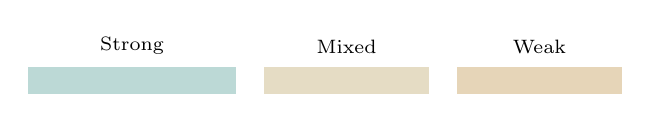
\begin{tikzpicture}[x=1cm,y=1cm]
  \fill[tsteal!28] (0,0) rectangle (2.65,0.34);
  \fill[ougold!35] (3.0,0) rectangle (5.1,0.34);
  \fill[tswarn!28] (5.45,0) rectangle (7.55,0.34);
  \node[anchor=south,font=\scriptsize] at (1.325,0.38) {Strong};
  \node[anchor=south,font=\scriptsize] at (4.05,0.38) {Mixed};
  \node[anchor=south,font=\scriptsize] at (6.5,0.38) {Weak};
\end{tikzpicture}
\end{center}
\end{frame}

\begin{frame}{7. External Benchmark Findings}
  \slidelead{Public benchmarks test whether the same evaluation logic still works outside our own synthetic setup.}
  \begin{columns}[T,totalwidth=\textwidth]
    \column{0.48\textwidth}
    \begin{block}{What this demonstrates}
      The system now runs on public tasks, not only internal tests.
    \end{block}
    \begin{block}{Interpretation}
      Traceability is already strong. Retrieval and answer quality remain the next clear optimization target.
    \end{block}
    \column{0.48\textwidth}
    \statcard{Aggregate TrustStack score}{63.09 / 100}
    \vspace{0.45em}
    \statcard{Task metric}{0.141}
    \vspace{0.45em}
    \statcard{Citation alignment}{83.8\%}
  \end{columns}
\end{frame}

\begin{frame}[shrink=2]{8. Validity and Next-Stage Readiness}
  \slidelead{The current version is a strong baseline: measurable, reproducible, and ready for stronger next-stage validation.}
  \begin{columns}[T,totalwidth=\textwidth]
    \column{0.49\textwidth}
    \begin{block}{What is already strong}
      \small
      \begin{itemize}
        \item Reproducible local runtime
        \item Explicit scoring and risk logic
        \item Real benchmark coverage
      \end{itemize}
    \end{block}
    \column{0.49\textwidth}
    \begin{block}{What comes next}
      \small
      \begin{itemize}
        \item stronger retrieval models
        \item richer human-study evaluation
        \item broader public benchmark coverage
      \end{itemize}
    \end{block}
  \end{columns}
\vspace{0.35em}
\begin{center}
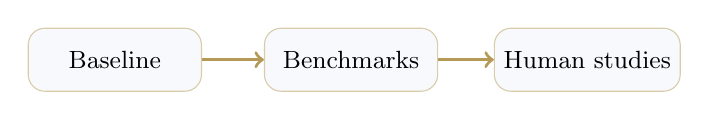
\begin{tikzpicture}[x=1cm,y=1cm]
  \node[draw=ouline, fill=tssoft, rounded corners=6pt, minimum width=2.2cm, minimum height=0.8cm] (a) at (0,0) {\small Baseline};
  \node[draw=ouline, fill=tssoft, rounded corners=6pt, minimum width=2.2cm, minimum height=0.8cm] (b) at (3.0,0) {\small Benchmarks};
  \node[draw=ouline, fill=tssoft, rounded corners=6pt, minimum width=2.2cm, minimum height=0.8cm] (c) at (6.0,0) {\small Human studies};
  \draw[ougold, line width=1.2pt, ->] (a) -- (b);
  \draw[ougold, line width=1.2pt, ->] (b) -- (c);
\end{tikzpicture}
\end{center}
\end{frame}

\begin{frame}{9. Conclusion}
  \slidelead{TrustStack makes AI trust easier to inspect, measure, and report.}
  \begin{block}{Main contribution}
    It connects live evidence review, formal scoring, benchmark evaluation, and report-ready artifacts into one coherent workflow.
  \end{block}
  \vspace{0.6em}
  \begin{columns}[T,totalwidth=\textwidth]
    \column{0.32\textwidth}
    \statcard{System role}{Evidence-first evaluator}
    \column{0.32\textwidth}
    \statcard{Empirical basis}{Synthetic + external}
    \column{0.32\textwidth}
    \statcard{Deliverable}{Report-ready artifacts}
  \end{columns}
  \vspace{0.6em}
  \begin{center}
    {\large\bfseries Questions}
  \end{center}
\end{frame}

\end{document}
